
\newcommand{\plotgoldensection}{%
	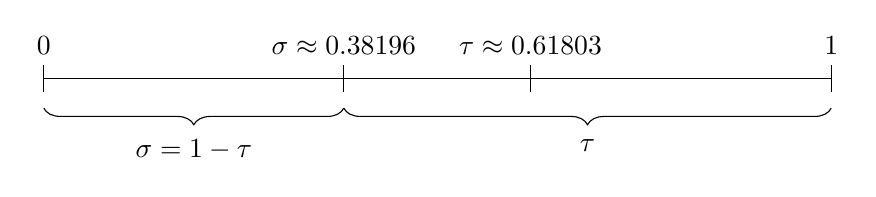
\begin{tikzpicture}
		\draw(0,0)--(10,0);
		\draw(0,-5pt)--(0,5pt) node[above] {$ 0 $};
		\draw(3.81,-5pt)--(3.81,5pt) node[above] {$ \sigma \approx 0.38196 $};
		\draw(6.18,-5pt)--(6.18,5pt) node[above] {$ \tau \approx 0.61803 $};
		\draw(10,-5pt)--(10,5pt) node[above] {$ 1 $};
		\draw[decorate, decoration={brace, mirror, amplitude=6pt}, yshift=-2.5ex] (0,0) -- node[below=1.8ex] {$ \sigma = 1 - \tau $} (3.81,0);
		\draw[decorate, decoration={brace, mirror, amplitude=6pt}, yshift=-2.5ex] (3.81,0) -- node[below=1.8ex] {$ \tau $} (10,0);
	\end{tikzpicture}
}

\newcommand{\plotsigmoid}{%
	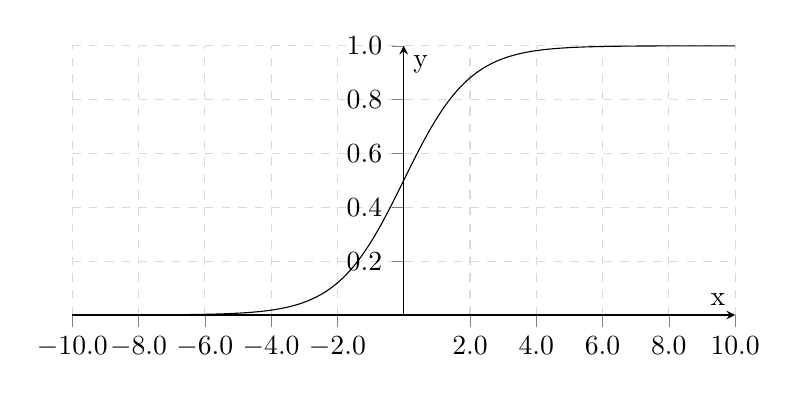
\begin{tikzpicture}
		\begin{axis}[
				legend pos=north west,
				axis x line=middle,
				axis y line=middle,
				x tick label style={/pgf/number format/fixed, /pgf/number format/fixed zerofill,
						/pgf/number format/precision=1},
				y tick label style={/pgf/number format/fixed, /pgf/number format/fixed zerofill,
						/pgf/number format/precision=1},
				grid = major,
				width=10cm,
				height=5cm,
				grid style={dashed, gray!30},
				xmin=-10,
				xmax= 10,
				ymin= 0,
				ymax= 1,
				axis background/.style={fill=white},
				xlabel=x,
				ylabel=y,
				tick align=outside,
				enlargelimits=false]
			\addplot[domain=-10:10,samples=500] {1/(1+exp(-x))};
			% \addlegendentry{$ \sigmoid(x) = \frac{1}{1+e^{-x}} $}
		\end{axis}
	\end{tikzpicture}
}

\newcommand{\plotvectorangle}{%
	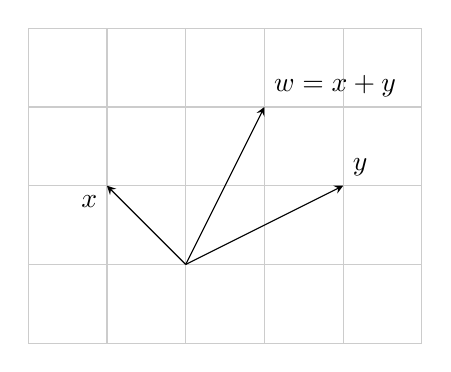
\begin{tikzpicture}
		\draw[thin,gray!40] (-2,-1) grid(3,3);
		\draw[-stealth](0,0) -- (-1,1) node[anchor=north east]{$\boldsymbol{x}$};
		\draw[-stealth](0,0) -- (2,1) node[anchor=south west]{$\boldsymbol{y}$};
		\draw[-stealth](0,0) -- (1,2) node[anchor=south west]{$\boldsymbol{w = x + y}$};
	\end{tikzpicture}
	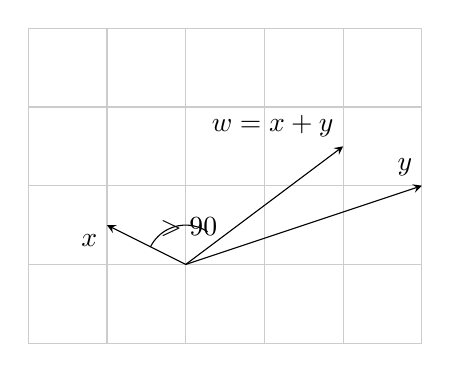
\begin{tikzpicture}
		\draw[thin,gray!40] (-2,-1) grid(3,3);
		\draw[-stealth](0,0) -- (-1,0.5) node[anchor=north east]{$\boldsymbol{x}$};
		\draw[-stealth](0,0) -- (3,1) node[anchor=south east]{$\boldsymbol{y}$};
		\draw[-stealth](0,0) -- (2,1.5) node[anchor=south east]{$\boldsymbol{w = x + y}$};
		\draw [black] (56.30:0.5) arc [start angle=56.30, end angle=153.43, radius=0.5cm]
		node [above right] {$ > \ang{90} $};
	\end{tikzpicture}
}
